\ifx\PREAMBLE\undefined
\documentclass{report}
\usepackage[format = hang, font = bf]{caption}
\usepackage{graphicx}
\usepackage{array}
\usepackage{amsmath}
\usepackage{mathtools}
\usepackage{boxedminipage}
\usepackage{listings}
\usepackage{makecell}%diagonal line in table
\usepackage{float}%allowing forceful figure[H]
\usepackage{xcolor}
\usepackage{amsfonts}%allowing \mathbb{R}
\usepackage{alltt}
\usepackage{algorithmicx}
\usepackage[chapter]{algorithm} 
%chapter option ensures that algorithms are numbered within each chapter rather than in the whole article
\usepackage[noend]{algpseudocode} %If end if, end procdeure, etc is expected to appear, remove the noend option
\usepackage{xspace}
\usepackage{color}
\usepackage{url}
\def\UrlBreaks{\do\A\do\B\do\C\do\D\do\E\do\F\do\G\do\H\do\I\do\J\do\K\do\L\do\M\do\N\do\O\do\P\do\Q\do\R\do\S\do\T\do\U\do\V\do\W\do\X\do\Y\do\Z\do\[\do\\\do\]\do\^\do\_\do\`\do\a\do\b\do\c\do\d\do\e\do\f\do\g\do\h\do\i\do\j\do\k\do\l\do\m\do\n\do\o\do\p\do\q\do\r\do\s\do\t\do\u\do\v\do\w\do\x\do\y\do\z\do\0\do\1\do\2\do\3\do\4\do\5\do\6\do\7\do\8\do\9\do\.\do\@\do\\\do\/\do\!\do\_\do\|\do\;\do\>\do\]\do\)\do\,\do\?\do\'\do+\do\=\do\#\do\-}
\usepackage[breaklinks = true]{hyperref}
\lstset{language = c++, breaklines = true, tabsize = 2, numbers = left, extendedchars = false, basicstyle = {\ttfamily \footnotesize}, keywordstyle=\color{blue!70}, commentstyle=\color{red!70}, frame=shadowbox, rulesepcolor=\color{red!20!green!20!blue!20}, numberstyle={\color[RGB]{0,192,192}}}
\mathchardef\myhyphen="2D
% switch-case environment definitions
\algblock{switch}{endswitch} 
\algblock{case}{endcase}
%\algrenewtext{endswitch}{\textbf{end switch}} %If end switch is expected to appear, uncomment this line.
\algtext*{endswitch} % Make end switch disappear
\algtext*{endcase}
\begin{document}
\fi
\chapter{Parsing}
The lexer takes a string of characters as input and transforms it into a string of tokens. A parser takes the string of tokens as input, and produces a parse tree. Sometimes the parse tree is just implicit and is not actually built. Also, some compilers finish the two tasks in one phase.
\section{Context free grammars}
\subsection{Introduction}
Not all strings of tokens are valid programs, which calls for a language for describing valid strings of tokens as well as a method to distinguish valid strings of tokens from invalid ones.

Programming languages have recursive structures: an {\bf expression} is often made up of other expressions. {\bf Context free grammars} are a natural notation for such structure.

A context free grammar consists of 
\begin{itemize}
\item a set of terminals  ($T$)
\item a set of non-terminals ($N$)
\item a start symbol ($S\in N$)
\item a set of productions ($P$)
\end{itemize}

A production is a relation of symbols:
\begin{equation}
X\rightarrow Y_1Y_2\dots Y_n
\end{equation}
in which $X\in N$, and $Y_i\in T\cup N\cup \{\varepsilon\}$. 

As an example, the language $\{(^i)^i\} ,i = 0,\dots,N$ can be expressed by the CFG with  $N = \{S\}, T = \{(,)\}$
and productions $\{S\rightarrow (S), S\rightarrow \varepsilon \}$.

Productions can be regarded as substitution rules. Terminals are so-called because there is no rule to replace them. Once generated, they are permanent. Terminals ought to be tokens of the programming language. Let $G$ be a CFG with start symbol $S$. The language $L(G)$ of $G$ is 
\begin{equation}
\{a_1\dots a_n|\forall a_i\in T, S\xrightarrow{*}a_1\dots a_n\}
\end{equation}
in which $S\xrightarrow{*}a_1\dots a_n$ means that $S$ can be rewritten into $a_1\dots a_n$ in a few steps with the substitution rules defined by the productions.

In the definition of production,  no precedence between operators or associativity of operator is assumed. For example, the grammar 
\begin{equation}\label{intops}
E\rightarrow E + E | E - E | E * E | E/E | (E) | int
\end{equation}
defines the normal $+-\times \div$ operations of integers, but do not assume the precedence of $\times \div$ over $+-$, or the normal left associativity of these operators.
\subsection{Derivations}
With the help of CFG, we are able to figure out whether a string of tokens belongs to a language. However, we would also like to know the structure of the string, i.e. the parse tree, which calls for the help of derivations.

A sequence of productions is called a derivation. It can be drawn as a tree. The start symbol is the tree's root, and for each production $X\rightarrow Y_1Y_2\dots Y_n$, $Y_1\dots Y_n$ is added as children of $X$. Such a tree drawn to describe an expression is called the {\bf parse tree} of the expression.

A parse tree has terminals at the leaves and non-terminals at the interior nodes. An in-order traversal of the leaves is the original input. The parse tree shows the association of operations, while the input string does not.

According to the order of the non-terminals being replaced, a derivation can be left-most or right-most, or of a random order, which is rarely used. Both the left-most and the right-most derivation have the same parse tree.
\subsection{Ambiguity}
A grammar is {\bf ambiguous} if it has more than one parse tree for some string. Equivantly, there is more than one left-most (right-most) derivation for this string. Ambiguity is a problem we strive to avoid. There are two solutions to the problem: either we directly rewrite the grammar unambiguously, or we enforce precedences on operations (e.g. * over +).

Here we give an example of rewriting grammar. The grammar
\begin{equation}
\text{E}\rightarrow \text{E}*\text{E} | \text{E}+\text{E} | (\text{E}) | id
\end{equation}
is ambiguous. 1 + 2 + 3 can be generated by \{1 + 2\} + 3 or 1 + \{2 + 3\}. It can be written as 
\begin{equation}
\begin{split}
\text{E}&\rightarrow \text{E}' + \text{E}\\
\text{E}'&\rightarrow id * \text{E}' | id | (\text{E}) * \text{E}' | (\text{E}),
\end{split}
\end{equation}
which is no longer ambiguous. In the new grammar, $E$ can generate sum(+), while $E'$ can generate product(*). \{1 + 2\} + 3 is no longer legal in the new grammar.

Consider the grammar
\begin{equation}
\begin{split}
\text{E}\rightarrow &\text{ if E then E}\\
|&\text{ if E then E else E}\\
|&\text{ OTHER}
\end{split}
\end{equation}
that decribes an ``if then else'' relation in which ``else'' is optional. It is ambiguous because the expression 
``if $E_1$ then if $E_2$ then $E_3$ else $E_4$'' has two parse trees because the ``else'' could correspond to both ``then''s. The parse tree of the previous expression could be either ``if $E_1$ then \{if $E_2$ then $E_3$ else $E_4\}$'' or ``if $E_1$ then \{if $E_2$ then $E_3$\} else $E_4$''We want to rewrite the grammar so that every ``else'' matches the cloest ``then''. The new grammar is
\begin{equation}
\begin{split}
\text{E}\rightarrow &\text{ MIF}\\
|&\text{ UIF}\\
\text{MIF}\rightarrow &\text{ if E then MIF else MIF}\\
|&\text{ OTHER}\\
\text{UIF}\rightarrow &\text{ if E then E}\\
|&\text{ if E then MIF else UIF}
\end{split}
\end{equation}
in which MIF means all ``then''s are matched, while UIF means some ``then''s are unmatched. In this new grammar, the second parse tree is no longer legal.

Unfortunately, it is impossible to automatically convert an ambiguous grammar to an unambiguous one. The manual conversion job is tedious, and the unambiguous grammar is often too complex to comprehend quickly. On the contrary, grammar with ambiguity is almost always tidy and more natural. But we need some mechanism to tackle the problem of ambiguity, which is the approach taken by most parsing tools. The most frequently used disambiguation mechanisms are precedence declarations and associativity declarations.

Note that the rewritten grammar no longer generates the same set of expressions from the point of view of semantic meaning. It only ensures that the same set of strings is generated. The grammar \eqref{intops} can be rewritten as 
\begin{equation}
\text{E}\rightarrow \text{E} + int |\text{E} - int | \text{E} * int |\text{E} / int | (E) | int
\end{equation}
to remove the ambiguity. However, 3 * 5 + 2 - 6 / 2 will be parsed as and only as \{\{\{3 * 5\} + 2\} - 6\} / 2, which is against normal precedence and associativity assumptions. In order to make the grammar work correctly in the intended way, simply rewriting the grammar is far from enough. It must be combined with other measures such as precedence and associativity definitions. 
\section{Error handling}
Compiler has two major tasks to complete: translating valid programs and detecting invalid ones. Different kinds of errors can be detected by different components of the compiler: lexcial errors by lexer, syntactic errors by parser and semantic errors by type checker. There are also errors that are not within the scope of the programming language, and thus remain to be found by the programmer through tests.

An error handler within the compiler is expected to 
\begin{itemize}
\item report errors accurately and clearly;
\item recover from an error quickly;
\item not slow down the compilation of valid codes.
\end{itemize}
There are three different approaches to implement the error handler: panic mode, error productions and automatic local/global correction. The first two are used in current compilers.

\subsection{Panic mode}
Panic mode is the simplest and thus the most popular method. When an error is detected, it discards tokens until one with a clear role is found, and resumes the compilation there. The ``clear'' token it looks for is usually the terminator of a statement or a funtion. In Bison (a popular parser generator), a special terminal {\sf error} is used to describe how much input to skip in case of an error. For example,
\begin{equation*}
\text{E}\rightarrow \text{E} + \text{E} | (\text{E}) | \text{error int}|\text{error}
\end{equation*}
specifies that an integer is regarded as a token to resume the compilation when an error occurs.
\subsection{Error productions}
Common errors made by programmers can sometimes be predicted. For example, 5 * x is often mistakenly written as 5 x. We can add new productions covering such typos into the grammar so that the compilation can continue, and the programmer receives warnings concerning the errors. This approach has an obvious disadvantage that it compilates the grammar.
\subsection{Automatic correction}
In the early years of programming, compilation is a time-consuming process. Programmers had to spent hours or even a whole day waiting for the compilation result. So compilers were expected to automatically correct probable errors in the program so that the time would not be totally wasted due to small mistakes such as typos, and more errors could be found in a single compilation cycle. This requirement makes it hard to implement a satisfactory compiler, and it also slows down the compilation of correct codes. Nowadays compilation is much more faster, and programmers tend to recompile everytime they fix an error. Thus complex error recovery becomes less compelling than a few decades ago.

\section{Top down parsing}
\subsection{Abstract syntax tree}
A parser traces the derivation of a sequence of tokens, but the rest of the compiler needs a structural representation of the program. {\bf Abstract syntax tree}, or {\bf AST} is the structure we use.

A parse tree traces operations of the parser and captures nesting structure of the token string being parsed. It contains a lot of verbose information, and the AST is an abstracted version that also captures the nesting structure, but is much more compact.

Consider the grammar $\text{E} \rightarrow \text{int} | (\text{E}) | \text{E + E}$ and the string 5 + (2 + 3). The parse tree and the related AST are shown in Figure \ref{parsetree} and Figure \ref{ast}.
\begin{figure}
\centering
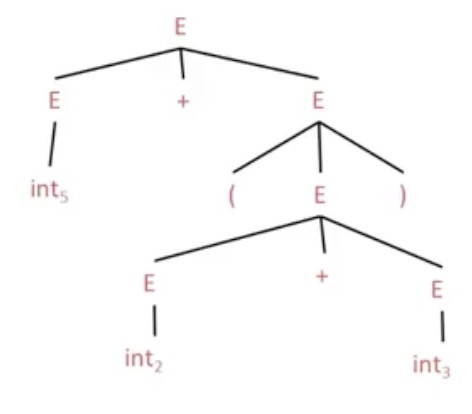
\includegraphics[width = 0.5\textwidth]{parsetree.jpg}
\caption{Parse tree of 5 + (2 + 3)}\label{parsetree}
\end{figure}
\begin{figure}
\centering
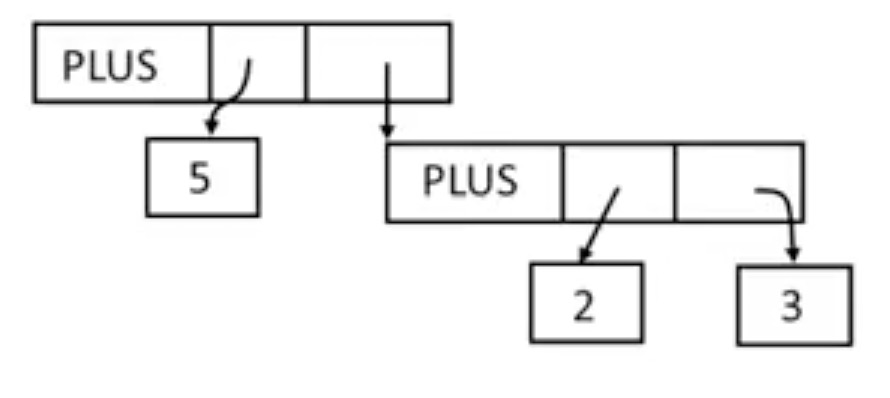
\includegraphics[width = 0.5\textwidth]{ast.jpg}
\caption{AST of 5 + (2 + 3)}\label{ast}
\end{figure}
\subsection{Recursive descent algorithm}
{\bf Recursive descent parsing} is a top-down parsing method, with which the parse tree is built from the top and from left to right. When building a parse tree, we start with the top-level non-terminal E, and try the rules of E in order. When another non-terminal is met, this process is carried out recursively. If a mis-match is found, we need to do the back tracking to find the correct rule to match.

Some rules in the illustration of the recursive descent parsing algorithm: TOKEN will be the type of tokens, and its instances will be INT (for int), OPEN (for `('), CLOSE (for `)'), TIMES (for `*'), etc; the global variable {\sf next} will point to the next token in the input.

Some boolean functions need to be defined to check matches of token terminals and CFG rules. For a given token terminal {\sf tok}, for the nth production of S, and for all productions of S, the functions are respectively 
\begin{lstlisting}[mathescape]
bool term(TOKEN tok) { return *next++ = tok; }
bool S$_n$() { $\dots$ }
bool S() { $\dots$ }
\end{lstlisting}

As an example, consider the grammar 
\begin{equation}\label{favgrammar}\begin{split}
\text{E}\rightarrow&\text{T }|\text{ T + E }\\\text{T}\rightarrow&\text{ int }|\text{ int * T }|\text{ (E).}
\end{split}\end{equation}
We will have
\begin{lstlisting}[mathescape]
bool E$_1$() { return T(); }
bool E$_2$() { return T() && term(PLUS) && E(); }
bool E() {
	TOKEN *save = next;
	return (next = save, E$_1$()) || (next = save, E$_2$());
}
bool T$_1$ = { return term(INT); }
bool T$_2$ = { return term(INT) && term(TIMES) && T(); }
bool T$_3$ = { return term(OPEN) && E() && term(CLOSE); }
bool T() {
	TOKEN *save = next;
	return (next = save, T$_1$()) || 
		   (next = save, T$_2$()) || 
		   (next = save, T$_3$());
}
\end{lstlisting}
To start the parser, {\sf next} needs to be set to the first token, and E() should be invoked. 

With the statement {\sf *save = next}, the current position is saved in {\sf save}. If the matching for a production succeeds, the matching for the whole non-terminal ends; otherwise {\sf next} is restored with {\sf next = save}, and the string continues to be matched with the next production. The use of the C++ comma operator is interesting.
\subsubsection{Limitations}
The recursive descent parsing algoruthm just presented is easy to be implemented by hand, but it is not general. Specificly for this example, consider the matching process for the string {\sf int * int}. We will go from E() to T() then to T$_1$(), which returns true and leaves us with the {\sf * int} segment. This segment cannot be matched, forcing us to wrongly reject the whole string. 

The problem is that with this algorithm, we have no way of back tracking and trying other productions once one production has been successfully matched. There exist a more general and yet more complex implementation that solves the problem by allowing ``full back tracking'', which will be covered later.
\subsubsection{Left recursion}
If a grammar has the form S$\rightarrow^+$S$\alpha$ for some $\alpha$, then it has a left recursion problem because the recursive descent matching process will end up in an infinite loop.

Left recursion problem can be solved by writing the algorithm. The grammar S$\rightarrow$S$\alpha|\beta$ that generates the language $\beta\alpha*$ can be rewritten as S$\rightarrow\beta$S', S'$\rightarrow\alpha\text{S'}|\varepsilon$. More generally, the grammar S$\rightarrow$S$\alpha_1|\dots|S\alpha_n|\beta_1|\dots|\beta_m$ that generates the language 
$(\beta_1|\dots|\beta_m)(\alpha_1|\dots|\alpha_n)*$ can be rewritten as S$\rightarrow\beta_1$S'$|\dots|\beta_m$S', S'$\rightarrow\alpha_1\text{S'}|\dots|\alpha_n\text{S'}|\varepsilon$. The general rule is to recognize the terminal rather than the non-terminal first when matching a combination of the two. 

There are algorithms that carries out the elimination of left recursion automatically (in the Dragon book).
\subsection{Predictive parsing}
Predictive parsing is another top-down parsing method. It is able to ``predict'' which production to use by looking at the next few tokens (lookahead) and no backtracking is needed. Predictive parser accepts so-called {\bf LL(k)} grammars which means {\bf left-to-right left-most-derivation} grammars requiring {\bf k} lookahead tokens. Here we will focus only on the case with k=1. Recall that in recursive descent, many choices of productions could be used at each step, and we use backtracking to undo the bad choices. But with LL(1) grammar, at most one production is available at each step. 

Consider the grammar \eqref{favgrammar}.  It is hard to predict the best production to use because for T, there are two productions that start with an {\sf int}, and for E, both productions start with T so that it is not clear how to make the predication. The grammar needs to be {\bf left-factored} in order to apply predicative parsing.

The new grammar is 
\begin{equation}\label{newgrammar}\begin{split}
\text{E}&\rightarrow\text{TX}\\
\text{X}&\rightarrow\text{+E }|\text{ }\epsilon\\
\text{T}&\rightarrow\text{int Y }|\text{ (E)}\\
\text{Y}&\rightarrow\text{* T }|\text{ }\epsilon
\end{split}\end{equation}
A {\bf LL(1) parsing table} can be generated according to this grammar as shown in Table \ref{ll1table}. The method to generate it will be covered later.
\begin{table}[ht]
\centering
\caption{Parsing table of grammar \eqref{newgrammar}}\label{ll1table}
\begin{tabular}{|c|c|c|c|c|c|c|}
\hline
& int & * & + & ( & ) & \$ \\\hline
E & TX & && TX&&\\\hline
X & && +E & & $\epsilon$ & $\epsilon$\\\hline
T & int Y &&& (E)&&\\\hline
Y && * T & $\epsilon$  && $\epsilon$  & $\epsilon$ \\\hline
\end{tabular}
\end{table}
\$ is the end of the input. Rows of the table represent the current leftmost non-terminal, while columns of the table represent the next input token. The entry is the rhs of the production to be used according to the combination of the leftmost non-terminal and the next input token. As an example, we have [E, int] = TX, which means that when the current non-terminal is E and the next input token is int, we should use the production E $\rightarrow$ TX. Also, [Y, +] = $\epsilon$ means that when the current non-terminal is Y and the next input token is +, the production Y $\rightarrow \epsilon$ should be used, i.e. Y should be got rid of. Finally, empty entry means that there is an error.

In order to carry out predictive parsing, we need to construct a stack that records the frontier of the parse tree. It contains non-terminals to be expanded as well as terminals to be matched. The top of the stack is always the leftmost pending terminal or non-terminal. The algorithm can be illustrated by Algorithm \eqref{preparalg}.
\begin{algorithm}
\caption{Predictive parsing algorithm}\label{preparalg}

\begin{algorithmic}
\State{Initialize stack = $<$S,\$$>$ and next}
\Repeat
\switch{ stack}
	\case{ $<$X,rest$>$:}
		\If{T[X, *next++] == $Y_1\dots Y_n$} 
			\State{stack$\gets <Y_1\dots Y_n$ rest$>$}
		\Else { error()} \EndIf \endcase
	\case{ $<$t,rest$>$:}
		\If{t == *next++} 
			\State{stack$\gets<$rest$>$}
		\Else { error()} \EndIf \endcase
\endswitch
\Until{stack == $<\text{ }>$}
\end{algorithmic}
\end{algorithm} 
If the stack is empty when we reach the end of the input, the string is accepted. If any error state is reached, the string is rejected. A step-by-step predictive parsing process of the string {\sf int * int} with the grammar \eqref{newgrammar} is shown in Table \ref{preparex}.
\begin{table}[ht]
\centering
\caption{Predictive parsing of int * int}\label{preparex}
\begin{tabular}{ccc}
\hline
Stack & Input & Action\\\hline
E\$ & int * int\$ & TX \\
TX\$ & int * int\$ & int Y\\
intYX\$ & int * int\$ & terminal\\
YX\$ & * int\$ & * T\\
*TX\$ & * int\$ & terminal\\
TX\$ & int\$ & int Y\\
intYX\$ & int\$ & terminal\\
YX\$ & \$ & $\epsilon$\\
X\$ & \$ & $\epsilon$\\
\$ & \$ & accept\\\hline
\end{tabular}
\end{table}

Now let's discuss the construction of LL1 parsing tables. For non-terminal A, production A$\rightarrow\alpha$ and terminal t, we will have T[A,t] = $\alpha$ in and only in two cases:
\begin{enumerate}
\item When $\alpha\xrightarrow{*}t\beta$, i.e. $\alpha$ can derive a t at the beginning. We say $t\in\text{First}(\alpha)$.
\item Otherwise when $\alpha\xrightarrow{*}\epsilon$ and $S\xrightarrow{*}\beta At\delta$. We say $t\in\text{Follow}(\alpha)$.
\end{enumerate}
\subsubsection{First set}
The formal definition of First(X) is 
\begin{equation}
\text{First}(X) = \{t|X\xrightarrow{*}t\alpha\}\cup\{\epsilon|X\xrightarrow{*}\epsilon\}.
\end{equation}
The algorithm to calculate First(X) is
\begin{enumerate}
\item For all terminal t, First(t) = \{t\}.
\item $\epsilon\in$ First(X) if $X\xrightarrow{*}\epsilon$, or if $X\xrightarrow{*}A_1\dots A_n$ and $\epsilon\in\bigcap\limits_j\text{First}(A_j)$.
\item $\text{First}(\alpha)\subseteq\text{First}(X)$ if $X\xrightarrow{*}A_1\dots A_n\alpha$ and $\epsilon\in\bigcap\limits_j\text{First}(A_j)$.
\end{enumerate}
For grammar \eqref{newgrammar}, we have 
\begin{itemize}
\item For terminals, First(t) = {t}, t = +, *, (, ), int.
\item First(T) = \{int, (\}
\item First(E) = \{int, (\}
\item First(X) = \{+, $\epsilon$\}
\item First(Y) = \{*, $\epsilon$\}
\end{itemize}
\subsubsection{Follow set}
The formal definition of Follow(X) is 
\begin{equation}
\text{Follow}(X) = \{t|S\xrightarrow{*}\beta Xt\delta\}.
\end{equation}
The algorithm to calculate Follow(X) is 
\begin{enumerate}
\item \$ $\in$ Follow(S)
\item For production $A\rightarrow\alpha X\beta$, First$(\beta) - \{\epsilon\}\subseteq$ Follow(X).
\item For production $A\rightarrow\alpha X\beta$ in which $\epsilon \in \text{First}(\beta)$, Follow(A) $\subseteq$ Follow(X).
\end{enumerate}
For grammar \eqref{newgrammar}, we have 
\begin{itemize}
\item Follow(E) = \{\$, )\}
\item Follow(X) = \{\$, )\}
\item Follow(T) = \{+,\$,)\}
\item Follow(Y) = \{+,\$,)\}
\item Follow('(') = \{int, (\}
\item Follow(')') = \{+,\$,)\}
\item Follow(int) = \{*,+,\$,)\}
\item Follow(+) = \{int, (\}
\item Follow(*) = \{int, (\}
\end{itemize}
\subsubsection{Parsing table}
To build a parsing table, for each production $A\rightarrow \alpha$, we need to do:
\begin{enumerate}
\item For each terminal $t\in\text{First}(\alpha)$, T[A, t] = $\alpha$.
\item If $\epsilon\in\text{First}(\alpha)$, for each terminal $t\in\text{Follow}(A)$, T[A, t] = $\alpha$.
\item If $\epsilon\in\text{First}(\alpha)$ and $\$\in\text{Follow}(A)$, T[A, \$] = $\alpha$.
\end{enumerate}

If any entry of the parsing table is multiple defined, then the grammar is nor LL(1). In particular, if the grammar is 
\begin{itemize}
\item not left factored
\item left recursive
\item ambiguous
\item $\dots$
\end{itemize}
then it is not LL(1). Actually most programming language CFGs are not LL(1). LL(1) grammar is too week to describe all the features required in these languages. 
\section{Bottom-up parsing}
Bottom-up parsing is more general than deterministic top-down parsing. Actually it is as efficient, and builds on all the ideas we have discussed in top-down parsing. Bottom-up parsing is the preferable method in reality. Bottom-up parsing does not require left-factored grammer, thus we can revert to the natural grammar \eqref{favgrammar} in the following discussion. Nonetheless, bottom-up parsers do not deal with ambiguous grammars, thus we still have to enforce precedence and associativity rules.

Bottom-up parsing reduces a string to the start symbol by inverting productions. As an example, consider the string int * int + int. It can be reduced to the start symbol E via the following path:
\begin{table}[H]
\centering
\begin{tabular}{ll}
int * int + int & T$\rightarrow$int\\
int * T + int & T$\rightarrow$int * T\\
T + int & T$\rightarrow$ int\\
T + T & E$\rightarrow$T\\
T + E & E$\rightarrow$T + E\\
E&\\
\end{tabular}
\end{table}
Obviously, the left column is the rightmost derivation of the string written in reverse. This is actually always true for bottom up parsers. {\bf Bottom-up parser traces a rightmost derivation in reverse.} It builds the parse tree from its leaves up towards the root, by combining smaller parse trees into larger ones.
\subsection{Shift reduce parsing}
Suppose $\alpha\beta\omega$ is a step of a bottom-up parse, and the next reduction to apply is $X\rightarrow\beta$. Since $\alpha X\omega\rightarrow\alpha\beta\omega$ is a step in a rightmost derivation, we can be sure that $\omega$ is a string of terminals. This inspires us of the idea of shift-reduce parsing. The string is split into two substrings, the right one unexamined by the parser, and the left one containing terminals and non-terminals. The dividing point is marked by a $|$ sign. Two actions are needed to carry out bottom-up parsing: \textbf{Shift} and \textbf{Reduce}. Shift means moving $|$ one place to the right, i.e. shifting one terminal to the left substring. Reduce means applying an inverse production at the right end of the left substring.

The left substring in shift-reduce string can be implemented by a stack, with the top of the stack being the $|$ sign. Each shift action pushes a terminal on the stack. Each reduce action pops symbols (rhs of the production rule, terminals and nonterminals) out of the  stack, and pushes a nonterminal on the stack. 

In a given state, more than one action might lead to a valid parse. If it is legal to shift or reduce, there is a \textbf{shift/reduce} conflict. If there are two legal reduces, then there is a \textbf{reduce/reduce} conflict. Reduce/reduce conflicts are always bad, indicating some serious problem of the grammar. Shift/reduce conflicts can usually be removed by precedence definitions.
\subsection{Handle \& viable predixes}
Reducing whenever we meet a rhs of production will probably cause incorrect results. For example, we cannot reduce int * int to T * int after the first shift according to the grammar \eqref{favgrammar}. We should only reduce when its result can still be reduced to the start symbol. A \textbf{handle} is a reduction that also allows further reductions back to the start symbol. For a rightmost derivation $S\xrightarrow{*}\alpha X\omega\rightarrow\alpha\beta\omega$, we say $\alpha\beta$ is a handle of $\alpha\beta\omega$. \textbf{In shift-reduce parsing, handles appear only at the top of the stack (never inside).} Handles are never to the left of the rightmost non-terminal. Thus shift-reduce moves are sufficient, and the $|$ sign never has to move left. Bottom-up parsing algorithms are based on recognizing handles.

\subsubsection{Recognizing handles}
Unfortunately there exists no known efficient algorithm to recognize handles. Nonetheless, there are good heuristics for guessing handles, and for some fairly large classes of CFGs, these heuristics always identify the handles correctly.
\begin{figure}[ht]
\centering
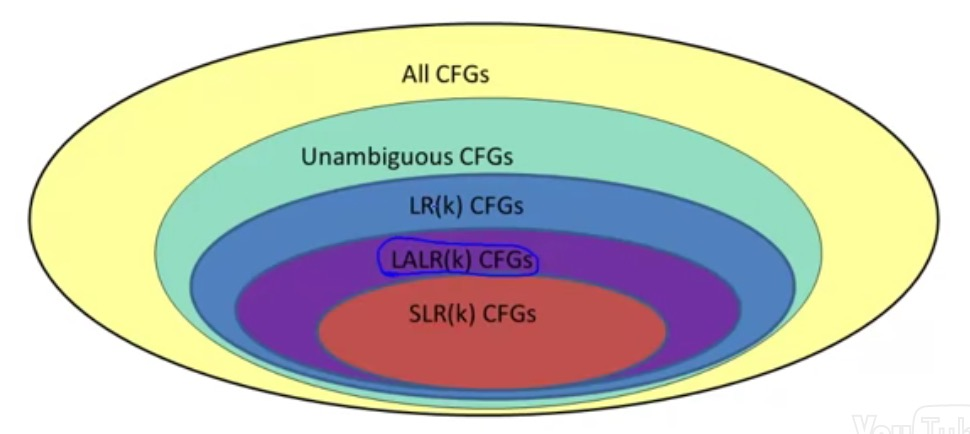
\includegraphics[width = 0.6\textwidth]{cfgvenn.jpg}
\caption{Relationship of different CFGs}\label{CFGsvenn}
\end{figure}
Figure \ref{CFGsvenn} illustrates the relationship of different kinds of CFGs. Most of the time we will talk about SLR(k) CFGs.

It is not obvious how to detect handles. We should always keep in mind that at each step, the parser sees only the stack and not the entire input, which is the starting point of the whole discussion. First we define a {\bf viable prefix}. $\alpha$ is a viable prefix if there is an $\omega$ such that $\alpha|\omega$ is a state of a shift-reduce parser. Here, $\alpha$ is the visible stack, while $\omega$ is the rest of the input. A viable prefix is a string that does not extend past the right end of the handle. It is called ``viable'' because it is a prefix of the handle. As long as the parser has viable prefixes on the stack, it means that no parsing error has been detected.

{\bf For any grammar, the set of viable prefixes is a regular language.} As a result, the set of viable prefixes can be recognized by a finite automaton. We will shown how to compute the automata that accept viable prefixes.

First we introduce the idea of an \textbf{item}. An item is a production with a $\cdot$\footnote{In the lectures . is used. I use $\cdot$(\LaTeX $\backslash$cdot) to avoid confusion with period.} somewhere in the rhs. For example, the production T$\rightarrow$(E) produces 4 items:  T$\rightarrow\cdot$(E), T$\rightarrow$($\cdot$E), T$\rightarrow$(E$\cdot$) and T$\rightarrow$(E)$\cdot$.For $\epsilon$-productions, the only item for X$\rightarrow\epsilon$ is X$\rightarrow\cdot$. Items are usually called the LR(0) items. They provide a description of intermediate steps of shirt-reduce parsing. Consider the input (int) for grammar \eqref{favgrammar}. (E$|$) is a state of a shift-reduce parse for it. (E is a prefix of the rhs of the production T$\rightarrow$(E), and it is to be reduced if a ) is recognized after the next shift. Item T$\rightarrow$(E$\cdot$) decribes such situation: we have seen (E and hope to see ).

The stack contains actually many prefixes of rhses of productions:
\begin{equation*}
\text{Prefix}_1\text{Prefix}_2\dots\text{Prefix}_{n-1}\text{Prefix}_{n}
\end{equation*}
Let Prefix$_i$ be a prefix of rhs of $X_i\rightarrow\alpha_i$. Prefix$_i$ will eventually reduce to $X_i$. In order that the parsing can continue, the missing part of $\alpha_{i-1}$ must start with $X_i$, i.e. there must exist a production $X_{i-1}\rightarrow\text{Prefix}_{i-1}X_i\beta$ for some $\beta$. Recursively $\text{Prefix}_{k+1}\dots\text{Prefix}_{n}$ eventually reduces to the missing part of $\alpha_k$.

Consider (int * int) for grammar \eqref{favgrammar}. (int * $|$ int) is a state of a shift-reduce parse. We have the stack of items:
\begin{equation*}
\begin{split}
\text{T}\rightarrow&\text{ (}\cdot\text{E)}\\\text{E}\rightarrow&\text{ }\cdot\text{T}\\\text{T}\rightarrow&\text{ int*}\cdot\text{T}
\end{split}\end{equation*}
\subsubsection{Recognizing viable prefixes}
As concluded previously, to recognize viable prefixes, we must recognize a sequence of partial rhses of productions, where each partical rhs can eventually reduce to part of the missing suffix of its predecessor. We will build an NFA that takes the stack as an input and decides whether to accept or reject it.
\begin{enumerate}
\item Add a dummy production S'$\rightarrow$S to the grammar G.
\item The NFA states are items of G, including the dummy production just added.
\item For item E$\rightarrow\alpha\cdot X\beta$, add transition
\begin{equation*}
\text{E}\rightarrow\alpha \cdot X\beta\xrightarrow{X}\text{E}\rightarrow\alpha X\cdot\beta
\end{equation*}
Here X is either a terminal or a non-terminal. This rule extends a prefix or an rhs.
\item For item E$\rightarrow\alpha\cdot X\beta$ and production $X\rightarrow\gamma$, add transition
\begin{equation*}
\text{E}\rightarrow\alpha \cdot X\beta\xrightarrow{\epsilon}X\rightarrow\cdot\gamma
\end{equation*}
Here X can only be non-terminals. This rule ends the current prefix and starts a new one.
\item Every state is an accepting state.
\item Start state is S'$\rightarrow$S. 
\end{enumerate}
Consider grammar \eqref{favgrammar}. After adding the dummy production, it becomes
\begin{equation}\begin{split}
\text{S'}\rightarrow&\text{ E}\\
\text{E}\rightarrow&\text{ T }|\text{ T + E }\\\text{T}\rightarrow&\text{ int }|\text{ int * T }|\text{ (E).}
\end{split}\end{equation}
By applying the algorithm above, we wind up with the NFA shown in Figure \ref{nfa}.
\begin{figure}[ht]
\centering
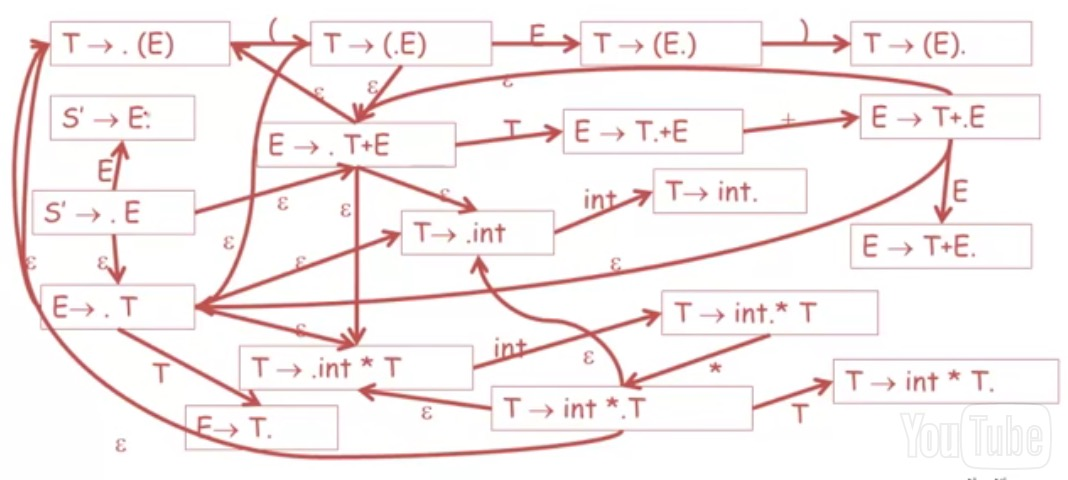
\includegraphics[width = \textwidth]{nfa.jpg}
\caption{NFA of grammar \eqref{favgrammar}}\label{nfa}
\end{figure}

The NFA gained using the algorithm above can be converted into a DFA. The states of the DFA are sets of items. The state of the DFA are called ``canonical collections of items (or LR(0) items)''\footnote{Dragon book provides another way to define LR(0) items.}.

The item X$\rightarrow\beta\cdot\gamma$ is said to be \textbf{valid} for a viable prefix $\alpha\beta$ if
\begin{equation*}
S' \xrightarrow{*}\alpha X\omega\rightarrow\alpha\beta\gamma\omega
\end{equation*}
by right-most derivation. After parsing $\alpha\beta$, the valid items are possible tops of the stack of items. An equivalent explanation is that for a given viable prefix $\alpha$, the valid items are exactly the items in the final state of the DFA after it reads that prefix.
\subsection{SLR parsing}
In this section we will present the {\bf SLR parsing} algorithm. SLR means ``simple left-to-right rightmost''.

First we will introduce a weak bottom-up parsing algorithm called LR(0) parsing. Suppose that the stack contains $\alpha$ and the next input is token t. The DFA on input $\alpha$ terminates in state s. Then the rules for shift-reduce actions are:
\begin{itemize}
\item Reduce by $X\rightarrow\beta$ if $X\rightarrow\beta\cdot\in s$
\item Shift if $X\rightarrow\beta\cdot t\omega\in s$. This is equivalent to the fact that s has a trasition labeled t.
\end{itemize}
LR(0) parsing has a reduce/reduce conflict if any state has two reduce items $X_1\rightarrow\beta_1\cdot$ and $X_2\rightarrow\beta_2\cdot$. It has a shift/reduce conflict if any state has a reduce item $X_1\rightarrow\beta_1\cdot$ and a shift item $X_2\rightarrow\beta_2\cdot t\delta$.

SLR improves on LR(0) shift/reduce heuristics. As a result, fewer shift/reduce conflicts will happen. The only adjustment is on the reduce rule, which is changed to 
\begin{itemize}
\item Reduce by $X\rightarrow\beta$ if $X\rightarrow\beta\cdot\in s$ and t$\in$Follow(X)
\end{itemize}
If any conflict still exists, then the grammar is not an SLR grammar. The handles of SLR grammars can be exactly detected by the heuristics. A lot of grammars are not SLR grammars. We can define define rules to resolve some confilicts for such grammars, which sometimes have the effect of precedence declaration.

Now we present the complete SLR parsing algorithm.
\begin{algorithm}[ht]
\caption{SLR parsing algorithm}\label{slrpar1}
\begin{algorithmic}
\State {Let M be the DFA for viable prefixes of G. and let $|x_1\dots x_n\$$ be the initial configuration. }
\Repeat
	\State{Let $\alpha|\omega$ be the current configuration and run M on the current stack $\alpha$.}
	\If{ M rejects $\alpha$} 
		\State{report parsing error}
	\Else 
		\State{M accepts $\alpha$ with items I, let a be the next input}
		\If {$X\rightarrow\beta\cdot a\gamma\in I$} shift
		\ElsIf {$X\rightarrow\beta\cdot \in I$ \textbf{and} $a\in$Follow(X)} reduce
		\Else { report parsing error} \EndIf
	\EndIf
\Until {configuration is $S|\$$}
\end{algorithmic}
\end{algorithm}

See video 8-6 for an exhaustive example of applying the algorithm.

Algorithm \eqref{slrpar1} can be improved because rerunning the viable predixes automaton is wasteful: reduce or shift will only change a few symbols on the top of the stack, while the rest of the stack stays the same, and the work on them is just a repeat. If the repeat can be avoided, the algorithm can run much more quickly. 

The state of the automaton on each prefix can be remembered. It will be more convenient to make the stack store $<$Symbol, DFA state$>$ pairs rather than just symbols. We will have a stack 
$$<\text{sym}_1,\text{state}_1>\dots<\text{sym}_n,\text{state}_n>,$$
in which state$_n$ is the final state of the DFA on sym$_1\dots$sym$_n$. The bottom of the stack is now $<$any, start$>$, in which any is any dummy state, while start is the start state of the DFA. The algorithm has 4 possible moves:
\begin{itemize}
\item Shift x. $<$a,x$>$ will be pushed on the stack, in which a is the current input, while x is a DFA state.
\item Reduce X$\rightarrow\alpha$. As before, pop the rhs elements off the stack and push the lhs on.
\item Accept.
\item Error.
\end{itemize}
We will define two parsing tables.
\begin{itemize}
\item Define \textsf{goto[i,A] = j} if state$_i\xrightarrow{A}$state$_j$. \textsf{goto} is just the transition function of the DFA.
\item Define \textsf{action[i,a]} for each DFA state $s_i$ and the next input terminal a.
\begin{itemize}
\item If $s_i$ contains item $X\rightarrow\alpha\cdot a\beta$ and \textsf{goto[i,a] = j} then \textsf{action[i,a] = shift j}.
\item If $s_i$ contains item $X\rightarrow\alpha\cdot$ and a$\in$Follow(X) and X$\neq$S' then \textsf{action[i,a] = reduce $X\rightarrow\alpha\cdot$}.
\item If $s_i$ contains item S'$\rightarrow$S, then \textsf{action[i,\$] = accept}.
\item Otherwise \textsf{action[i,a] = error}.
\end{itemize}\end{itemize}
The improved algorithm is shown in Algorithm \eqref{slrpar2}.
\begin{algorithm}[ht]
\caption{Improved SLR parsing algorithm}\label{slrpar2}
\begin{algorithmic}
\State {Let I = w\$ be the initial input}
\State {Let j = 0. }
\State {Let DFA state 1 have item S'$\rightarrow$S.}
\State {Let stack = $<$dummy, 1$>$}
\Repeat
	\switch{ action[top\_state(stack), I[j]]}
	\case { Shift k:}
		\State Push $<$I[j++], k$>$ on stack
	\endcase
	\case { reduce $X\rightarrow A$:}
		\State Pop $|A|$ pairs
		\State Push $<$X, goto[top\_state(stack), X]$>$ on stack
	\endcase
	\case { accept:} 
		\State Halt normally
	\endcase
	\case { error:}
		\State Halt with an error
	\endcase
	\endswitch
\Until {configuration is $S|\$$}
\end{algorithmic}
\end{algorithm}

In practice, SLR parsing is too simple and sometimes naive. LR(1), or LALR(1), which is based on LR(1) and includes some optimisations, parsing is much more widely used. The main difference between LR(1) and SLR is that LR(1) builds lookahead into the items. An LR(1) items looks like [T$\rightarrow\cdot$int * T, \$], which means ``after seeing int * T, reduce if lookahead is \$''. This mechanism is more accurate that using just the follow set to decide whether to reduce.

\ifx\PREAMBLE\undefined
\end{document}
\fi